\chapter{Ising model}
\label{ch:ising}
\index{Ising model}

The Ising model is the first model through the machinery of
Chapter~\ref{ch:statmech}, worked end to end. Its results are new here, and
the published work it is checked against --- the Bethe critical temperature, and
the motif calculations of \citet{yoon2011} --- is cited where used. It comes first for two reasons:
its answer on a graph is already known, so every step can be checked against it;
and its result here is a sign that goes the other way from the obvious one.

Clustering \emph{lowers} the critical temperature at fixed degree, and it does
so even though a triangle transmits \emph{more} per traversal than a link does.
Both halves hold, and they pull in opposite directions.
Section~\ref{sec:magnetisation} substitutes the same interior into
Sec.~\ref{sec:response}'s magnetisation and susceptibility, where it closes
twice against textbook answers; Sec.~\ref{sec:clustering} is then the
accounting, on a null model where all three quantities are exact. There the two effects come apart: clustering
costs the transition temperature and buys a steeper rise out of it.
Section~\ref{sec:isingfive} runs the whole of it over the five structures of
Fig.~\ref{fig:mappings}, one paragraph each, where the accounting turns out to
matter more than the structure does.

\section{Spins inside complexes}
\label{sec:spins}

Put an Ising spin $\sigma_{i}=\pm1$ on every node, couple every pair inside
every complex, and write down the partition function the rest of the chapter
differentiates:
\begin{equation}
  \begin{aligned}
    \mathcal{H}&=-J\sum_{a}\ \sum_{\{i,j\}\subset a}\sigma_{i}\sigma_{j}
              \;-\;B\sum_{i}\sigma_{i},\\
    Z&=\sum_{\{\sigma\}}e^{-\beta\mathcal{H}},
    \qquad
    f=-\frac{1}{\beta N}\ln Z,
  \end{aligned}
  \label{eq:Hising}
\end{equation}
the first sum over complexes, the second over nodes, and $N$ the number of
nodes. A complex of cardinality $c$ therefore carries $\binom{c}{2}$ bonds,
and a graph is the case $c=2$ where each carries one. The external field $B$ is
zero except where Sec.~\ref{sec:response} differentiates $f$ with respect to
it; it is written $B$ rather than $h$ because $h$ is the cavity field of
Eq.~\eqref{eq:up}, the busiest symbol in Part~III, and because
Chapter~\ref{ch:introduction} introduced the field under that letter.
Where a $B$ carries two layer indices, or stands inside $\det(I-B)$, it is
the branching matrix of Eq.~\eqref{eq:branch} and not a field.

The Ising model on graph ensembles with prescribed motifs has been treated
directly \citep{yoon2011}; the point here is that no separate treatment is
needed. That is the entire model specification, and everything else is
Chapter~\ref{ch:statmech}: Eq.~\eqref{eq:emitted} with Eq.~\eqref{eq:Hising}
inside it gives $u'$, Eq.~\eqref{eq:branch} gives the transition, and squaring
$u'$ gives the de Almeida--Thouless line instead. The calculation is $L\times L$
linear algebra with an enumeration of size $2^{c}$ behind each entry, and
nothing about it had to be invented for this chapter.

\section{What a complex transmits}
\label{sec:transmits}
\index{transmission factor}

Writing $t=\tanh\beta J$, the interior sum gives
\begin{equation}
  \begin{aligned}
    c=2:&\quad u'=t,\\
    c=3:&\quad u'=t/(1-t+t^{2}),\\
    c=4:&\quad u'=(t+t^{3})/(1-2t+3t^{2}),
  \end{aligned}
  \label{eq:uclique}
\end{equation}
with no useful closed form beyond, but exact by enumeration at any cardinality
small enough to enumerate --- which is the same condition the rest of the
formalism already lives under.

By Eq.~\eqref{eq:emitted},
\[
  u'=\frac{\partial}{\partial h_{1}}\tfrac12\bigl[\ln Z(+)-\ln Z(-)\bigr]
     \bigg|_{h=0}
    =\tfrac12\Bigl[\ave{\sigma_{1}}_{+}-\ave{\sigma_{1}}_{-}\Bigr],
\]
the two averages taken inside the complex at zero cavity field with $\sigma_{0}$
held at $+1$ and at $-1$.

For $c=3$ with $a=\beta J$, the interior energy
$\sigma_{0}\sigma_{1}+\sigma_{0}\sigma_{2}+\sigma_{1}\sigma_{2}$ takes the value
$3$ on the one configuration where both others agree with $\sigma_{0}$, and
$-1$ on the other three. So
\[
  \ave{\sigma_{1}}_{+}=\frac{e^{3a}-e^{-a}}{e^{3a}+3e^{-a}}
                      =\frac{e^{4a}-1}{e^{4a}+3},
\]
and $\ave{\sigma_{1}}_{-}=-\ave{\sigma_{1}}_{+}$ by spin-flip symmetry. Hence
$u'=(e^{4a}-1)/(e^{4a}+3)$, and substituting $e^{2a}=(1+t)/(1-t)$,
\[
  u'=\frac{(1+t)^{2}-(1-t)^{2}}{(1+t)^{2}+3(1-t)^{2}}
    =\frac{4t}{4-4t+4t^{2}}=\frac{t}{1-t+t^{2}}.
\]
The same enumeration at $c=4$ gives the third line of
Eq.~\eqref{eq:uclique}, and beyond that the expressions stop being worth
writing down. \code{Chygraph.\allowbreak u\_\allowbreak prime} returns them, over
\code{ising.\allowbreak clique\_\allowbreak derivative} for the closed forms and
\code{cavity.\allowbreak cavity\_\allowbreak derivative} for the enumeration they
are checked against.

The first half of the chapter's result follows at once, and it is the intuitive
half. Since $t/(1-t+t^{2})>t$ on $0<t<1$, and $(t+t^{3})/(1-2t+3t^{2})$ is larger
still, \emph{a triangle transmits more to each of its members than an
independent edge does} (Fig.~\ref{fig:transmit}). The extra route --- round the
third corner --- is real, and it is precisely the loop that a tree-based
calculation on the underlying graph could not have kept.

\begin{figure}[t]
\centering
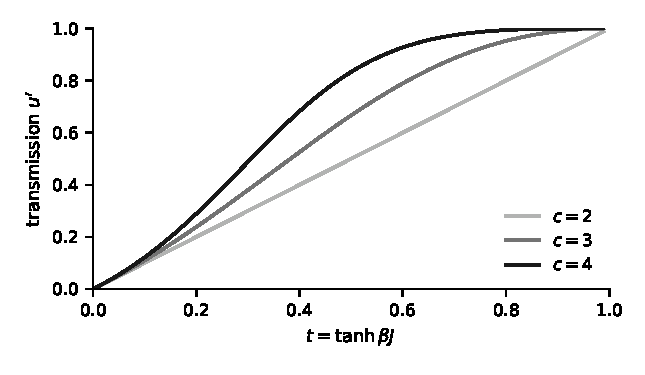
\includegraphics[width=0.88\linewidth]{figs/fig-transmit.pdf}
\caption{\textbf{More per traversal.} The transmission $u'$ of
Eq.~\eqref{eq:uclique} against $t=\tanh\beta J$. The $c=2$ curve is the
diagonal $u'=t$; larger complexes lie above it, because a member can be reached
around the inside of the complex as well as directly. At leading order in $t$
all three coincide, so the enhancement is $O(t^{2})$ --- which is why
Sec.~\ref{sec:clustering}'s effect decays with degree. Generated by
\code{figs/\allowbreak ising.\allowbreak py}.}
\label{fig:transmit}
\end{figure}

It would be natural to conclude that clustering favours order. It does not, and
Sec.~\ref{sec:clustering} is why.

\section{The critical temperature}
\label{sec:tc}
\index{critical temperature|textbf}

Substituting Eq.~\eqref{eq:uclique} into Eq.~\eqref{eq:branch} and turning the
handle, structure by structure.

On a graph the condition is
\begin{equation}
  \ave{\kbar}\,\tanh\beta J=1,
  \label{eq:tcgraph}
\end{equation}
which is Eq.~\eqref{eq:tc-intro} --- the textbook Bethe result, and the
reassurance one wants before trusting anything else in the chapter. It is also
Chapter~\ref{ch:potts}'s $\tau_{2}(2,v)\ave{\kbar}=1$, the same line reached
along a third route.

On a network of $c$-cliques it is $\ave{\kbar}(c-1)u'(c)=1$, and on a graph
with links and triangles it is Eq.~\eqref{eq:LT}. Neither needs a closed form to
be evaluated. At chy-degree two, a single clique layer gives Table~\ref{tab:cliquetc}.
\begin{table}[t]
\centering\small
\begin{tabular}{lccccc}
\hline\hline
$c$ & $2$ & $3$ & $4$ & $5$ & $6$\\
\hline
$\beta J_{c}$ & $0.5493$ & $0.2118$ & $0.1304$ & $0.0940$ & $0.0734$\\
AT line & $0.8814$ & $0.4024$ & $0.2670$ & $0.2015$ & $0.1625$\\
\hline\hline
\end{tabular}
\caption{\textbf{One clique layer at chy-degree two.} The critical coupling from $\ave{\kbar}(c-1)u'(c)=1$, and the de Almeida--Thouless coupling from the same condition with $u'$ replaced by $u'^{2}$, against cardinality. Generated by \code{figs/\allowbreak ising.\allowbreak py}.}
\label{tab:cliquetc}
\end{table}
with the second row anticipating Sec.~\ref{sec:atline}.

\paragraph{Over several layers.} Those are the one- and two-layer cases of one
formula, and it is worth having in general because three of
Fig.~\ref{fig:mappings}'s five structures carry more than one layer.
Equation~\eqref{eq:branch} puts $\ave{\kbar}_{m}$ on the diagonal and
$\ave{\kappa}_{m}$ off it and multiplies both by the same
$(c_{m}-1)u'(c_{m})$, so $B$ is a rank-one matrix plus a diagonal,
$B=\mathbf{1}v^{\!\top}+\mathrm{diag}(d)$ with
$v_{l}=\ave{\kappa}_{l}(c_{l}-1)u'(c_{l})$ and
$d_{l}=(\ave{\kbar}_{l}-\ave{\kappa}_{l})(c_{l}-1)u'(c_{l})$. A matrix of that
shape has a scalar determinant condition, so $\det(I-B)=0$ is
\begin{equation}
  \sum_{l}\frac{\ave{\kappa}_{l}(c_{l}-1)\,u'(c_{l})}
               {1-\bigl(\ave{\kbar}_{l}-\ave{\kappa}_{l}\bigr)(c_{l}-1)\,u'(c_{l})}
  =1,
  \label{eq:tcmulti}
\end{equation}
one term per layer and an eigenvalue problem no longer. At one layer the
$\ave{\kappa}$'s cancel and it is $\ave{\kbar}(c-1)u'(c)=1$, which is
Eq.~\eqref{eq:tcgraph} at $c=2$; at two layers, expanded, it is
Eq.~\eqref{eq:LT}. With Poisson layers every $\ave{\kbar}_{l}=\ave{\kappa}_{l}$,
every $d_{l}$ vanishes, and it flattens further to
$\sum_{l}\ave{\kappa}_{l}(c_{l}-1)u'(c_{l})=1$: the layers add, and nothing but
the sum survives.

\section{Magnetisation and susceptibility}
\label{sec:magnetisation}
\index{magnetisation}
\index{susceptibility}
\index{critical amplitude}

Section~\ref{sec:response} took the two observables either side of the
transition for an arbitrary interior: the order parameter
Eq.~\eqref{eq:magclosure} and the response Eq.~\eqref{eq:chi}, with the
exponents $\beta=1/2$ and $\gamma=1$ and the two amplitudes
Eqs.~\eqref{eq:magamp} and~\eqref{eq:chiamp}, in the same external field $B$
as Eq.~\eqref{eq:Hising}. Substituting the Ising interior into them is this
section, and it costs what substituting into Eq.~\eqref{eq:branch} cost in
Sec.~\ref{sec:tc}: an enumeration and nothing else.

\paragraph{What the interior supplies.} Equation~\eqref{eq:a1a3} asks for two
cumulants of the interior magnetisation $S$, and for the all-pairs clique they
are had from the same enumeration as Sec.~\ref{sec:transmits}. The first is
$a_{1}=(c-1)u'$ with $u'$ of Eq.~\eqref{eq:uclique}, so nothing new is computed
for it. The second has a closed form at $c=2$: expanding
$\bar u(h)=\mathrm{atanh}(t\tanh h)$ gives
\begin{equation}
  a_{3}=\tfrac{1}{3}\,t\,(t^{2}-1),
  \label{eq:a3edge}
\end{equation}
negative on $0<t<1$ because a bond saturates, which is the condition
Eq.~\eqref{eq:magamp} needs to have a continuous branch at all. Above $c=2$ it
is a number from the enumeration, as $u'$ is.

\paragraph{The susceptibility on a graph.} One layer at $c=2$ with $u'=t$
reduces Eq.~\eqref{eq:chi} to $\chi=1+\ave{k}t/(1-\ave{\kbar}t)$. For a
$k$-regular graph $\ave{\kbar}=k-1$ and this is
\begin{equation}
  \chi=\frac{1+t}{1-(k-1)t},
  \label{eq:chibethe}
\end{equation}
the Bethe-lattice susceptibility; for a Poisson degree, its own excess, it is
$\chi=1/(1-\ave{k}t)$. Both are textbook, and both come out of
Eq.~\eqref{eq:chi} without adjustment --- which is the reassurance this chapter
wants before trusting the same expression on a clique layer.
Equation~\eqref{eq:chiamp} then collapses to $A_{\chi}=T_{c}/(k-2)$.

\paragraph{The amplitude on a graph.} Equation~\eqref{eq:magamp} likewise
closes at $c=2$:
\begin{equation}
  A_{m}=\frac{k}{k-1}\sqrt{\frac{3(k-1)J}{T_{c}}},
  \label{eq:magampgraph}
\end{equation}
which returns $2.3548$ at $k=4$. As $k$ grows $T_{c}\to J(k-1)$ and
$A_{m}\to\sqrt3$, the Curie--Weiss amplitude of the fully connected magnet: the
second check from outside, and the one that says the machinery reduces to mean
field where it has to.

\section{Clustering lowers \texorpdfstring{$T_{c}$}{Tc}}
\label{sec:clustering}
\index{clustering!and the critical temperature|textbf}
\index{null model}

Equation~\eqref{eq:branch} carries a \emph{multiplicity} as well as a
transmission, and the two move in opposite directions. The accounting between
them is what follows.

Arrive at a degree-$n$ vertex of a graph along one of its links. Then $n-1$
further links branch away. Arrive at the same vertex through one of its $n/2$
triangles, and only $n-2$ branch --- because one of the two neighbours in the
triangle just traversed is already accounted for, its influence sitting inside
$u'$ rather than being counted again as a separate route.

More per branch, fewer branches. Which wins is arithmetic. At $n=4$ the two
conditions are $3t=1$ for links and $2u'_{\triangle}=1$ for triangles, so at the
link ensemble's critical coupling $t=1/3$ the triangle enhancement would have to
carry $u'$ from $1/3$ to $1/2$ to break even. It reaches
\begin{equation}
  u'_{\triangle}\bigl(t=\tfrac13\bigr)
    =\frac{1/3}{1-\tfrac13+\tfrac19}=\frac{3}{7},
\end{equation}
which is not enough. The lost branch wins, and the network of triangles needs to
be colder before it orders.

\paragraph{Against a null model that is actually matched.} The comparison has to
be stated carefully, and this book has said why in four places already ---
Secs.~\ref{sec:promoting}, \ref{sec:helporhurt}, \ref{sec:joint}
and~\ref{sec:epidemics-lessons}: naming what is held fixed is most of the work. The unambiguous null is regular. Take an
$n$-regular graph against a network of $n/2$ triangles per vertex. These have
identical degree distribution $p_{d}=\delta_{d,n}$, identically neutral degree
correlations, and the same number of edges per vertex. They differ in one thing
only: whether those edges close into triangles (Table~\ref{tab:trianglenull}).
\begin{table}[t]
\centering\small
\begin{tabular}{rrrr}
\hline\hline
$n$ & $T_{c}$ links & $T_{c}$ triangles & change\\
\hline
$4$ & $2.8854$ & $2.4853$ & $-13.9\%$\\
$6$ & $4.9326$ & $4.7209$ & $-4.3\%$\\
$8$ & $6.9521$ & $6.8052$ & $-2.1\%$\\
$10$ & $8.9628$ & $8.8498$ & $-1.3\%$\\
$20$ & $18.9824$ & $18.9296$ & $-0.3\%$\\
\hline\hline
\end{tabular}
\caption{\textbf{Clustering lowers $T_{c}$ at fixed degree.} An $n$-regular graph against a network of $n/2$ triangles per vertex: identical degree distribution, identically neutral degree correlations, the same number of edges per vertex, differing only in whether those edges close into triangles. The effect is largest at low degree and dies as $1/n^{2}$: the last column is $-1/(n-1)^{2}$ to within seven per cent from $n=6$ upward. Generated by \code{figs/\allowbreak ising.\allowbreak py}.}
\label{tab:trianglenull}
\end{table}
The effect is large at low degree and dies as $1/n^{2}$, and the second power
is the point. Each of the two competing terms is $O(1/n)$ on its own: the branch
that was lost is one out of $n-1$, and the transmission enhancement, $O(t^{2})$
by Fig.~\ref{fig:transmit} with $t\sim1/n$ at the transition, is a fraction
$O(t)$ of $t$ itself. They cancel at that order. Solving the two conditions
exactly --- $(n-1)t=1$ for links, $t^{2}-(n-1)t+1=0$ for triangles --- leaves
$\Delta T_{c}/T_{c}=-1/(n-1)^{2}+O(n^{-3})$, which is $-4.0$, $-2.0$, $-1.2$ and
$-0.28$ per cent at $n=6$, $8$, $10$ and $20$ against the table's $-4.3$, $-2.1$,
$-1.3$ and $-0.3$. The absolute shift dies as $1/n$, since $T_{c}\simeq n-1$; it
is the fractional effect that is a square.

\paragraph{The comparison that misleads.} It is the one a careful person
reaches for first. Take a Poisson layer of $n$ links
against a Poisson layer of $n/2$ triangles. This matches the \emph{mean} degree
and nothing else. The triangle construction gives degree $d=2X$ with
$X\sim\mathrm{Poisson}(n/2)$, so $d$ is even, its variance is $2n$ rather than
$n$, and its excess degree is $\ave{\bar k}=n+1$ rather than $n$: the control is
the less heterogeneous of the two, not the matched one.
Equation~\eqref{eq:branch} sees that through the multiplicity. A Poisson layer
is its own excess, so the triangle layer carries
$(c-1)\ave{\kbar}_{\triangle}=2\cdot n/2=n$, which is exactly the link layer's
$\ave{\kbar}_{|}=n$. The branch that was lost in the regular comparison is not
lost here, only the transmission enhancement survives, and the apparent sign
reverses --- at $n=4$, $T_{c}=4.7209$ for the triangles against $3.9152$ for the
links. Read instead against a configuration model carrying the triangle
ensemble's own excess degree $n+1$, the link layer gives $4.9326$ and the sign
is the one the regular comparison found.

Figure~\ref{fig:clustering} runs the comparison continuously rather than at two
points. Give a vertex $k_{\triangle}=fn/2$ triangles and $k_{|}=(1-f)n$ links,
so that its degree is exactly $n$ for every $f$ and the whole family shares one
degree distribution; $f$ is then the fraction of a vertex's neighbours reached
through a triangle, and the local clustering coefficient is $f/(n-1)$. $T_{c}$
falls monotonically with $f$ at every degree.

\begin{figure}[t]
\centering
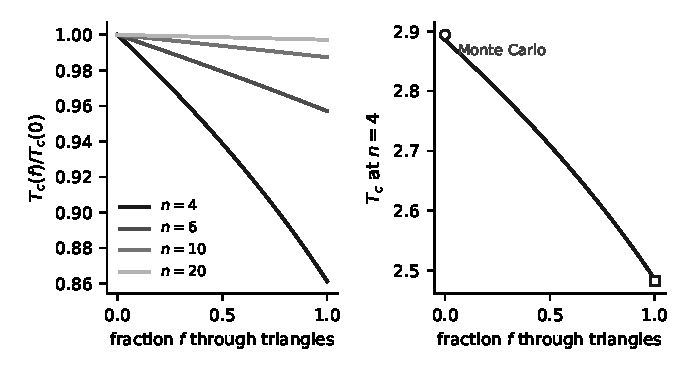
\includegraphics[width=\linewidth]{figs/fig-clustering.pdf}
\caption{\textbf{Clustering lowers $T_{c}$ at fixed degree.} A vertex carries
$fn/2$ triangles and $(1-f)n$ links, so every member of the family has degree
exactly $n$ and the same $p_{d}$; only the clustering coefficient, $f/(n-1)$,
varies. Left: $T_{c}(f)/T_{c}(0)$ from Eq.~\eqref{eq:branch}. The fall is
monotone at every degree and shrinks as the degree grows. Right: the same
family at $n=4$ in absolute units, with the Wolff cluster simulations of
Eq.~\eqref{eq:mc} at $f=0$ and $f=1$ --- open symbols, and they use no cavity
equation. Generated by \code{figs/\allowbreak ising.\allowbreak py}.}
\label{fig:clustering}
\end{figure}

\paragraph{What this does and does not show.} It does not show that a degree
distribution is uninformative. The two ensembles are distinguishable
--- by their clustering coefficient, if by nothing else. What it shows is that
no configuration model on the same degree distribution reproduces the triangle
ensemble's $T_{c}$, and that Eq.~\eqref{eq:uclique} supplies the difference in
closed form. The quantity missing from $\{p_{d},e_{dd'}\}$ is the size of the
shift, and Chapter~\ref{ch:introduction} promised exactly that debt would be
paid here.

\paragraph{The test from outside.} All of the above is one formalism talking to
itself. The check that is not is a direct simulation. Wolff cluster updates on
a $4$-regular random graph and on a network of two triangles per vertex --- the
first row of the table, every vertex at degree exactly $4$ in both --- give
Binder cumulant crossings
\begin{equation}
  T_{c}^{\mathrm{links}}=2.894,
  \qquad
  T_{c}^{\mathrm{tri}}=2.482,
  \label{eq:mc}
\end{equation}
at $n=3000$ and $12000$, against $2.8854$ and $2.4853$ from
Eq.~\eqref{eq:branch}: agreement to $0.30$ and $0.13$ per cent, and a measured shift
of $-14.2$ per cent against a predicted $-13.9$. Both the sign and the size survive
contact with something that has never heard of a cavity equation.

\paragraph{The same null, one order up.} The matched null above carries
Sec.~\ref{sec:magnetisation}'s two observables without change, both of its
members being regular: an $n$-regular graph against a network of $n/2$
triangles per vertex, identical degree distribution either way. Clustering
lowers $T_{c}$ and \emph{raises} both amplitudes
(Table~\ref{tab:amplitudenull}).
\begin{table}[t]
\centering\small
\begin{tabular}{rrrrrrr}
\hline\hline
$n$ & $A_{m}$ links & $A_{m}$ tri. & change & $A_{\chi}$ links & $A_{\chi}$ tri. & change\\
\hline
$4$ & $2.3548$ & $2.8368$ & $+20.5\%$ & $1.4427$ & $1.9883$ & $+37.8\%$\\
$6$ & $2.0926$ & $2.2370$ & $+6.9\%$ & $1.2332$ & $1.3488$ & $+9.4\%$\\
$8$ & $1.9863$ & $2.0572$ & $+3.6\%$ & $1.1587$ & $1.2098$ & $+4.4\%$\\
$10$ & $1.9285$ & $1.9708$ & $+2.2\%$ & $1.1204$ & $1.1493$ & $+2.6\%$\\
$20$ & $1.8241$ & $1.8335$ & $+0.5\%$ & $1.0546$ & $1.0605$ & $+0.6\%$\\
\hline\hline
\end{tabular}
\caption{\textbf{Clustering raises both amplitudes at fixed degree.} The null of Table~\ref{tab:trianglenull}, an $n$-regular graph against a network of $n/2$ triangles per vertex, now read one order up: $A_{m}$ of Eq.~\eqref{eq:magamp} and $A_{\chi}$ of Eq.~\eqref{eq:chiamp}. Both gaps shrink with degree, as the $T_{c}$ gap of Table~\ref{tab:trianglenull} does, and for the same reason. Generated by \code{figs/\allowbreak ising.\allowbreak py}.}
\label{tab:amplitudenull}
\end{table}
The two statements are consistent and it is worth saying why. What the
paragraphs above weighed was multiplicity against transmission at the
transition, and the multiplicity won, so $T_{c}$ fell. The amplitudes are
weighed below the transition, where the lost branch has already been paid for
in the position of $T_{c}$ and what is left is the transmission: at its own
critical temperature the triangle network is the more strongly coupled of the
two per branch, and it leaves the transition faster. So the triangle network
orders at a lower temperature and, once it orders, rises out of the transition
more steeply and responds to a field more strongly. Both gaps die with degree
exactly as the temperature gap does.

\begin{figure}[t]
\centering
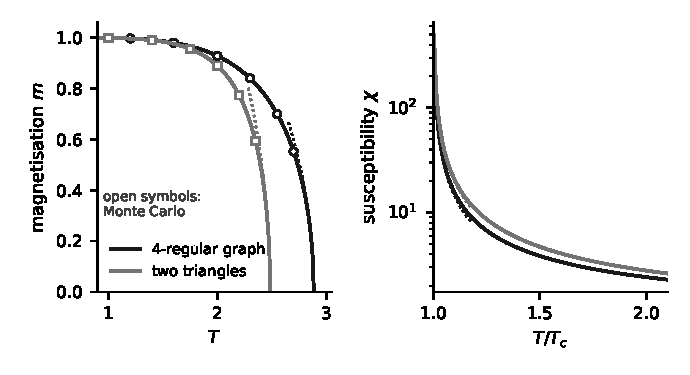
\includegraphics[width=\linewidth]{figs/fig-magnetisation.pdf}
\caption{\textbf{The order parameter and the response.} The matched pair of
this section --- a $4$-regular graph and a network of two triangles
per vertex, degree exactly four in both. Left: the magnetisation from
Eq.~\eqref{eq:magclosure}, with the square-root asymptote
Eq.~\eqref{eq:magamp} dotted and the Wolff simulations of
Eq.~\eqref{eq:mc} as open symbols. Right: the susceptibility from
Eq.~\eqref{eq:chi} against reduced temperature, with the $\gamma=1$ asymptote
Eq.~\eqref{eq:chiamp} dotted; both diverge at their own $T_{c}$, and the
triangle curve lies above because its amplitude is larger. Generated by
\code{figs/\allowbreak ising.\allowbreak py}.}
\label{fig:magnetisation}
\end{figure}

\paragraph{The whole branch, not one point.} Equation~\eqref{eq:magclosure} is
a curve rather than a single temperature, so the Wolff simulations above test
more of the theory than they were run for. The same runs that gave the Binder
crossings give $\ave{m^{2}}^{1/2}$ at every
temperature on the ordered side, and over six temperatures on each structure,
from $T/T_{c}=0.40$ up to $0.95$, the closed form and the simulation agree to
$0.06$ per cent or better at $n=12000$. Nothing in the simulation knows what a
cavity equation is, and the agreement is over the whole branch and not at one
point.

\section{Structured networks}
\label{sec:isingfive}

Chapter~\ref{ch:chygraphs} claimed that one calculation covers the five
structures of Fig.~\ref{fig:mappings}. Sections~\ref{sec:hsfive}
and~\ref{sec:fivecover} pay that out for hitting set and for vertex cover,
where the observable is a threshold in density and the list splits by
cardinality. Here the observable is a temperature and the list barely splits at
all: under the matched null of Sec.~\ref{sec:clustering} the six rows of
Table~\ref{tab:fiveising} take two values, and the sixth lies between them.

That is Eq.~\eqref{eq:tcmulti} doing the work. The condition is one sum over
layers, so a layer list is read off term by term, and two lists with the same
terms give the same temperature however the terms are grouped into structures.

\begin{table}[t]
\centering\small
\begin{adjustbox}{max width=\linewidth}
\begin{tabular}{lccrrr}
\hline\hline
structure & $c$ & $\kappa$ & $T_{c}$ & $T_{c}$ Poisson & AT\\
\hline
A graph & $2$ & $6$ & 4.9326 & 5.9440 & 2.0781\\
A hypergraph & $3$ & $3$ & 4.7209 & 6.8052 & 2.4853\\
A multiplex network & $2,2$ & $3,3$ & 4.9326 & 5.9440 & 2.0781\\
Interacting graphs & $2,2,2$ & $2,2,2$ & 4.9326 & 5.9440 & 2.0781\\
Interacting hypergraphs & $3,3,3$ & $1,1,1$ & 4.7209 & 6.8052 & 2.4853\\
A clustered graph & $2,3$ & $2,2$ & 4.7952 & 6.5400 & 2.3407\\
\hline\hline
\end{tabular}

\end{adjustbox}
\caption{\textbf{The five structures at one degree.} Regular layers, $\kappa$
complexes of each layer per vertex, chosen so that every row sits at degree
exactly six and the six share a degree distribution --- the matched null of
Sec.~\ref{sec:clustering}. $T_{c}$ is Eq.~\eqref{eq:tcmulti}; \emph{AT} is the
same with $u'^{2}$, anticipating Sec.~\ref{sec:atline}. The \emph{Poisson}
column is the identical layer lists with the excess chy-degree left equal to
the mean, which matches the mean degree and nothing else: it reverses the sign,
and is the comparison Sec.~\ref{sec:clustering} warns about. Generated by
\code{figs/\allowbreak ising.\allowbreak py:table\_\allowbreak five\_\allowbreak structures}.}
\label{tab:fiveising}
\end{table}

\paragraph{A graph} is one layer of links. Every $u'$ is $t=\tanh\beta J$ and
there is one term, so Eq.~\eqref{eq:tcmulti} is $\ave{\kbar}\,t=1$, which is
Eq.~\eqref{eq:tcgraph}. For example, the $6$-regular random graph has
$\ave{\kbar}=5$, so $t=1/5$ and $T_{c}=4.9326$. That is the Bethe value, and
the row the others are read against.

\paragraph{A hypergraph} is one complex layer with the cardinality free. Where
that layer carries a single size $c$, which is how every layer in
Chapters~\ref{ch:ising}--\ref{ch:cover} is built, the single term gives
$\ave{\kbar}(c-1)u'(c)=1$ --- the multiplicity $c-1$ against the transmission
$u'(c)$, which is Sec.~\ref{sec:clustering}'s accounting on one line. Where it
carries a distribution of sizes instead, Eq.~\eqref{eq:sbaru}'s size-biased
average takes the place of $(c-1)u'(c)$ and nothing else moves. For
example, a network of triangles at three per vertex, meeting only at vertices so
that the degree is again six, has $\ave{\kbar}=2$, and $2\cdot2\,u'(3)=1$ gives
$T_{c}=4.7209$: the same degree arranged into cliques instead of links, and
colder by $4.3$ per cent. This row is
not a new calculation --- it is the $n=6$ line of Table~\ref{tab:trianglenull},
which is Sec.~\ref{sec:clustering}'s result, arrived at here as one entry in a
list rather than as the chapter's headline.

\paragraph{A multiplex network} is $L$ link layers on the same vertices. Every
layer has $c=2$, so every $u'$ is the same $t$ and Eq.~\eqref{eq:tcmulti} is
\[
  \sum_{l}\frac{\ave{\kappa}_{l}\,t}
                {1-\bigl(\ave{\kbar}_{l}-\ave{\kappa}_{l}\bigr)t}=1,
\]
which is as far as one gets without saying what the degree distribution is. Two
conventions close it. With Poisson layers every
$\ave{\kbar}_{l}=\ave{\kappa}_{l}$, the denominators are $1$, and it is
$Kt=1$ with $K=\sum_{l}\ave{\kappa}_{l}$ the total number of links at a
vertex; with regular layers $\ave{\kbar}_{l}=\ave{\kappa}_{l}-1$, every
denominator is $1+t$, and it is $(K-1)t=1$. Either way only $K$ survives, so a
multiplex is the graph of the same total degree, whatever $L$ is and however the
links are shared out. For example, two $3$-regular link layers give $K=6$, so
$(K-1)t=1$ and $T_{c}=4.9326$, the graph's number exactly. An Ising spin cannot read a layer label, and what
Eq.~\eqref{eq:Hising} sees is the union; that the formalism keeps the layers
apart and still returns one number is the check, not the result.

\paragraph{Interacting graphs and hypergraphs} is $L$ layers whose cardinalities
need not agree --- one layer per interacting structure and a cross layer per
interacting pair, each free to have its own size. In general nothing
simplifies: Eq.~\eqref{eq:tcmulti} stands as it is, one term per layer, and the
layer list is substituted into it. Where the cardinalities do agree, all equal
to $c$, one $u'$ is shared and the previous paragraph goes through with
$(c-1)u'(c)$ in place of $t$:
\[
  \text{Poisson: } K(c-1)\,u'(c)=1,
  \qquad
  \text{regular: } (K-1)(c-1)\,u'(c)=1 ,
\]
so interacting layers of a single cardinality behave as one layer of that
cardinality carrying the total chy-degree. For example, three $2$-regular link
layers give $K=6$ and the graph's $4.9326$; three triangle layers at one
triangle per vertex give $K=3$ and the hypergraph's $4.7209$. So the panel adds
nothing here, and the nothing is worth recording. In Chapters~\ref{ch:hittingset}
and~\ref{ch:cover} the cross layer decides which side of a line the structure
falls on --- whether the hard field is exact there, whether a core-free branch
survives. Equation~\eqref{eq:tcmulti} has no line to fall either side of: a
cross layer contributes its own term to the sum, and the sum is all there is.
The panel that carried the most weight in the two neighbouring chapters carries
the least in this one.

\paragraph{A clustered graph} is a link layer together with one layer per clique
size the graph contains, which is Sec.~\ref{sec:everything}'s mapping. Two
cardinalities or more mean two or more different $u'$ and there is no collapse
to be had: Eq.~\eqref{eq:tcmulti} keeps one term per layer, and at two layers,
expanded, it is Eq.~\eqref{eq:LT}. For example, two links and two triangles per vertex,
degree six for the last time, sits at $4.7952$, between the two. It is Fig.~\ref{fig:clustering}'s family at
$f=2/3$: four of a vertex's six neighbours reached through a triangle, and a
temperature two-thirds of the way from the link value to the triangle one.
Nothing in the row is new either. What the list adds is that the family
Fig.~\ref{fig:clustering} draws is not a special construction but the generic
row --- every structure with more than one cardinality lands inside the
interval, and only the pure ones land on its ends.

\paragraph{The column that misleads.} The Poisson column of
Table~\ref{tab:fiveising} is the warning of Sec.~\ref{sec:clustering}, met again
as a property of the list rather than of one comparison. Leave the excess chy-degree equal to the mean and
every row rises, but the clique rows rise further --- $6.8052$ against $5.9440$
--- and the sign of the whole table reverses. Nothing about the structures has
changed. What changed is that matching the mean degree of a triangle ensemble to
a link ensemble does not match its excess, and Eq.~\eqref{eq:tcmulti} reads the
excess. A reader who built this table without Sec.~\ref{sec:clustering} in front
of them would conclude that clustering raises $T_{c}$ in four of the six rows.

\paragraph{What the list establishes.} Less than the two neighbouring sections
and in a more useful direction. Less, because there is no line for the
structures to fall either side of: Eq.~\eqref{eq:tcmulti} is a single sum, every
structure evaluates it, and the differences between the five are differences of
a few per cent rather than of kind. More useful, because that is the honest
shape of the claim for a thermodynamic observable, and because the one thing the
table does discriminate --- the matched null against the unmatched one --- is not
a property of the chygraph at all. It is a property of the comparison, and it
costs more of the answer here than cardinality does.

\section{The de Almeida--Thouless line}
\label{sec:atline}
\index{de Almeida--Thouless line|textbf}

Section~\ref{sec:replicas} listed three signals that a replica-symmetric answer
has stopped being right, and the first was the stability of the symmetric
solution itself. On a chygraph it costs one character.

Perturb the messages and ask whether the perturbation grows. A perturbation of
\emph{random} sign is transmitted with $u'$ and its effect measured by squaring,
so the relevant condition replaces $\ave{u'}$ by $\ave{u'^{2}}$ everywhere in
Eq.~\eqref{eq:branch} --- and nothing else moves, because the reweighting of
Eq.~\eqref{eq:reweight} is elementwise. On a graph the ferromagnetic line
$\ave{\kbar}t=1$ becomes $\ave{\kbar}t^{2}=1$, both textbook, and on any
chygraph the same substitution serves.

Since $u'\in(0,1)$ gives $u'^{2}<u'$, the spin-glass instability always requires
the stronger coupling: the second row of Sec.~\ref{sec:tc}'s table exceeds the
first at every cardinality, so it is reached only at the lower temperature. For a ferromagnet that is the expected ordering
and the line is not reached, the system ordering first. It becomes the operative
condition when the couplings carry random signs, and it is what
Chapter~\ref{ch:hittingset} will need when its own symmetric solution stops
being trustworthy.

\section{A different interaction inside the complex}
\label{sec:unanimity}
\index{unanimity interaction|textbf}
\index{spinodal}

Nothing in Chapter~\ref{ch:statmech} fixed what is inside a complex.
Equation~\eqref{eq:emitted} sums whatever Hamiltonian is put there and the
chy-degree step never sees it. So a different higher-order interaction is a
substitution rather than a new theory, and this section is the demonstration
that the claim is not empty.

Where Eq.~\eqref{eq:Hising} couples every pair inside a complex, let a hyperedge
instead lower the energy only when \emph{all} its members agree
\citep{son2026}:
\begin{equation}
  \mathcal{H}=-\sum_{e}J_{q}\,\delta_{\{\sigma_{i}\}_{i\in e}}
              -B\sum_{i}\sigma_{i},
  \label{eq:simH}
\end{equation}
with $\delta$ equal to one on the two unanimous states of a hyperedge and zero
on the other $2^{q}-2$. This is the interaction
Chapter~\ref{ch:epidemics} met as a threshold contagion rule --- a group that
acts only when everybody in it acts.

Write the rule as $1+(e^{a}-1)\delta$, $a=\beta J_{q}$, splitting the interior
sum into a free part and one correction. With cavity fields
$h_{1},\dots,h_{q-1}$ on the other members,
\[
  Z(\sigma_{0})=\prod_{j=1}^{q-1}\bigl(2\cosh h_{j}\bigr)
                +(e^{a}-1)\,e^{\sigma_{0}\sum_{j}h_{j}},
\]
the correction surviving only where every $\sigma_{j}=\sigma_{0}$.
Differentiating at $h=0$, the first term contributes nothing and
\[
  u'=\frac{e^{a}-1}{2^{\,q-1}+e^{a}-1}.
\]
Two remarks. This is elementary at \emph{any} cardinality, where the all-pairs
clique of Sec.~\ref{sec:transmits} needs an enumeration --- so a harder-looking
interaction can be easier inside. And at $q=2$ it is $\tanh(a/2)$: a unanimous
pair is an ordinary bond of half the coupling, as
$\delta_{\sigma_{0}\sigma_{1}}=(1+\sigma_{0}\sigma_{1})/2$ requires.

One trap. The equation above is the derivative with respect to \emph{one} other
member's field, the same convention as Eq.~\eqref{eq:uprime}, so the
multiplicity $q-1$ is supplied by Eq.~\eqref{eq:branch} and not here.
Differentiating instead with respect to a field common to all $q-1$ others
multiplies it by $q-1$; using \emph{that} in Eq.~\eqref{eq:branch} counts the
multiplicity twice. \code{Chygraph.\allowbreak simplicial} returns both: \code{emitted} is the
interior and \code{spinodal} the condition built on it, in the module
\code{simplicial}.

\paragraph{The infinite-connectivity limit.} Take one layer of cardinality $q$
at fixed chy-degree $k$ and impose \citeauthor{son2026}'s normalisation
$J_{q}=q/k$. Expanding the spinodal condition $(k-1)(q-1)u'=1$ in $1/k$,
\begin{equation}
  T^{*}\longrightarrow\frac{q(q-1)}{2^{\,q-1}}
  \qquad(k\to\infty),
  \label{eq:BW}
\end{equation}
which is their mean-field result, approached with residual
\begin{equation}
  T-T^{*}=-\frac{C_{q}}{k}+O(k^{-2}),
  \qquad
  C_{q}=\frac{q\bigl(2q-2^{\,q-1}\bigr)}{2^{\,q}}.
  \label{eq:Cq}
\end{equation}
Equation~\eqref{eq:BW} is non-monotonic in cardinality, peaking at $q=3$ and
$q=4$ together (Fig.~\ref{fig:unanimity}), and at finite chy-degree the
degeneracy is lifted. The coefficient $C_{q}$ vanishes when
$2q=2^{\,q-1}$, that is at $q=4$ and nowhere else. The leading
finite-connectivity correction is absent at exactly the cardinality that is
tricritical in the mean-field theory, so $T^{*}$ is approached there as $1/k^{2}$
rather than $1/k$ --- $-2.2\times10^{-5}$ at $k=200$ against
$-3.8\times10^{-3}$ at $q=3$.

\begin{figure}[t]
\centering
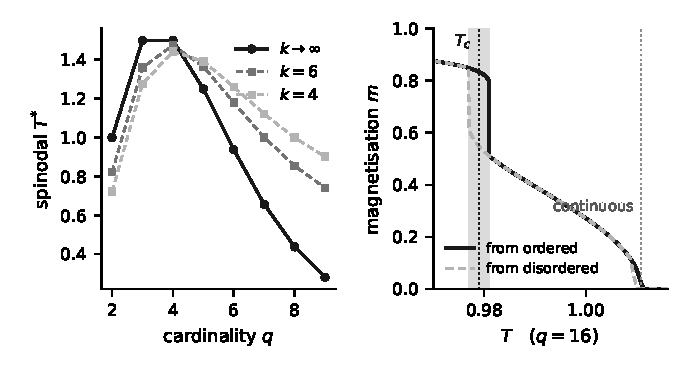
\includegraphics[width=\linewidth]{figs/fig-unanimity.pdf}
\caption{\textbf{A different interior, and a warning.} Left: the spinodal
against cardinality for the unanimity rule under the normalisation
$J_{q}=q/k$, at chy-degrees $4$ and $6$ and in the limit
Eq.~\eqref{eq:BW}. It is non-monotonic, and finite connectivity shifts where it
peaks. Right: the double transition at $q=16$ with
$(J_{q},J_{2},k_{q},k_{2})=(0.3,0.7,4,4)$, continued from an ordered and from a
disordered start. The continuous transition sits at $T=1.0108$; inside the
shaded coexistence window the two branches differ, and the free energies cross
at $T_{c}=0.9790$, where $m$ jumps by $0.286$. Generated by
\code{figs/\allowbreak ising.\allowbreak py}.}
\label{fig:unanimity}
\end{figure}

\paragraph{Where the branching condition stops being the transition.} For this
model, most of the interesting range is discontinuous, and there
Eq.~\eqref{eq:det} locates a spinodal rather than a transition. This is the
fourth time the book has arrived here --- Sec.~\ref{sec:breakdown} for
interdependent networks, Sec.~\ref{sec:groupcontagion} for threshold contagion,
Sec.~\ref{sec:transmission} for the Potts model above $q=2$ --- and it is the
first time the tool built in Sec.~\ref{sec:freeenergy} is actually used.

The right-hand panel of Fig.~\ref{fig:unanimity} is the calculation done
properly. At $q=16$ with $(J_{q},J_{2},k_{q},k_{2})=(0.3,0.7,4,4)$ there are two
transitions. The upper one is continuous, at $T=1.0108$, and it is essentially
the pairwise value: $u'$ is $O(2^{-q})$ at $q=16$, so the higher-order layer
contributes nothing to the linear instability. The lower one is first order. Iterating from a magnetised start and from a near-zero one, the two
branches differ on $0.9770<T<0.9810$; comparing Eq.~\eqref{eq:bethe} between
them inside that window, they cross at
\begin{equation}
  T_{c}=0.9790,\qquad \Delta m=0.286,
\end{equation}
with $m$ jumping from $0.548$ to $0.834$, and $T^{*}<T_{c}<T^{**}$ as it must.

\paragraph{A test that has to be done carefully.} Whether the transition at a
given $(q,k)$ is continuous or discontinuous is the sort of question that
invites a quick answer and is easy to get wrong. Iterating from an ordered start just
above the spinodal and finding a non-zero magnetisation looks like evidence of
coexistence --- but just above a \emph{continuous} transition the ordered branch
decays so slowly that a finite iteration budget reports exactly the same thing.
Critical slowing down mimics a first-order window.

Done properly --- a converged branch, a coexistence window of non-negligible
width, and a free-energy crossing strictly inside it --- the boundary sits
between $q=5$ and $q=6$ at chy-degree $3$, and between $q=4$ and $q=5$ from
chy-degree $4$ upward. Low connectivity delays the discontinuity by one in
cardinality and then stops mattering. At chy-degree $4$ and $q=5$, for instance,
the window is $1.1138<T<1.1308$ and the free energies cross at $T_{c}=1.1262$:
narrow, but real. At $q=4$ the apparent window is thirty times narrower and
holds no crossing at all, at chy-degree $4$, $6$, $10$ or $40$. That is the
difference between an artefact and a transition, and it is only visible if one
looks for the crossing.

\section{Checks}
\label{sec:ising-checks}

\checkhead{Known results}
On a graph the condition $\ave{\kbar}\tanh\beta J=1$ is the textbook Bethe
temperature, and Sec.~\ref{sec:tc}'s $u'$ is Chapter~\ref{ch:potts}'s
$\tau_{c}(2,v)$, checked in Sec.~\ref{sec:statmech-checks}.
With the Ising interior substituted, Eq.~\eqref{eq:chi} returns the
Bethe-lattice susceptibility Eq.~\eqref{eq:chibethe} on a regular graph and
$1/(1-\ave{k}t)$ on a Poisson one, to eleven digits at three couplings each;
both are textbook. Equation~\eqref{eq:magamp} reduces to
Eq.~\eqref{eq:magampgraph}, checked to $10^{-8}$ at $k=3,4,6,10$, and tends to
the Curie--Weiss value $\sqrt3$ as the degree grows --- $1.7338$ at $k=1000$
against $1.7321$. Equation~\eqref{eq:BW}'s infinite-connectivity limit
$T^{*}\to q(q-1)/2^{q-1}$ is \citeauthor{son2026}'s mean-field value, recovered
here by expanding the spinodal condition in $1/k$.

\checkhead{New results}
The rest of the chapter has no published counterpart.
Equation~\eqref{eq:uclique} is checked against the numerical enumeration behind
Eq.~\eqref{eq:emitted} at four couplings for $c=2,3,4$, and the closed form for
the unanimity rule likewise. Equation~\eqref{eq:tcmulti} reduces to
Eq.~\eqref{eq:LT} on expanding its two-layer case, and is checked against the
Perron root of Eq.~\eqref{eq:branch} to $10^{-9}$ on each of
Table~\ref{tab:fiveising}'s six layer lists. That table's graph and hypergraph
rows are the $n=6$ line of Table~\ref{tab:trianglenull} reached by the other
route; its three cardinality-two rows are checked to agree, its two pure-clique
rows likewise, and the mixed row to lie between them.
The two amplitudes are Sec.~\ref{sec:response}'s and are checked there; what
this chapter adds to them is the interior. Equation~\eqref{eq:a1a3}'s cumulants
are checked twice for the all-pairs clique: $a_{1}$ against the transmission
$(c-1)u'$ the threshold already uses, to twelve digits at $c=2,\dots,5$, and
$a_{3}$ against Eq.~\eqref{eq:a3edge} at $c=2$ and against finite differences of
the enumeration itself above it. And Eq.~\eqref{eq:magclosure} reproduces the
whole ordered branch, not one point: against the Wolff simulations at $n=12000$
it agrees to $0.06$ per cent or better at six temperatures on each of the two
structures of Sec.~\ref{sec:clustering}, from $T/T_{c}=0.40$ to $0.95$. That is
the one test of the order parameter from outside the formalism. Equation~\eqref{eq:Cq} is checked against the
spinodal computed from Eq.~\eqref{eq:det} at $k=200$ for $q=2,\dots,8$,
including the case $q=4$ where the prediction is that the correction
\emph{vanishes} and the residual duly falls to $2\times10^{-5}$. Carrying the
message as a distribution and iterating a population of samples --- the up step
a Poisson-compound convolution, the down step Eq.~\eqref{eq:emitted} evaluated
numerically --- gives $\beta J_{c}=0.164628$ against the closed-form $0.168236$
for a graph at six neighbours, and $0.144343$ against $0.146947$ for the
corresponding triangle network; independently, the gap between the ordered and
paramagnetic branches of Eq.~\eqref{eq:bethe} is zero to machine precision below
the transition and lifts off above it, in the same place. And
Eq.~\eqref{eq:mc}: the Wolff simulations use no cavity equation and confirm both
the sign and the size of the clustering effect. That is the only number in the
chapter that could have come out differently.

\checkhead{Partial results}
Equation~\eqref{eq:magclosure} carries Sec.~\ref{sec:response}'s restriction
into this chapter: it covers the two ends of Fig.~\ref{fig:clustering}'s family
and none of its interior, whose members give a vertex a fractional number of
triangles. Checking the closure against a population on a \emph{regular}
chygraph tests the excess bookkeeping of both routes and not the physics of
either, because a regular chygraph collapses the population onto one value; the
Monte Carlo above is the check that is not of that kind.
The population dynamics is low by $2.1$ and $1.8$ per cent, for a definite reason ---
a finite sweep budget calls a slowly decaying magnetisation ordered, which is
the same effect as the trap in Sec.~\ref{sec:unanimity} --- so it confirms the
closed forms rather than competing with them. Nothing here is evidence that the
treelike assumption holds on a real network: both simulated ensembles were built
so that their triangles share at most one atom, which is the condition the
theory needs and which Chapter~\ref{ch:data} showed real networks violate.
Chapter~\ref{ch:overlap} measures what that violation costs.
